\section{Week 2}
\textbf{\large Extended Surfaces: Fins}
\begin{itemize}
    \item Fin Equation:
    \begin{align*}
        \frac{d^2\theta}{dx^2} - m^2 \theta &= 0 \\
        \text{where } \; \theta &= T - T_{\infty} \\
        m^2 &= \frac{hp}{k A_c}
    \end{align*}
    \begin{figure}[H]
        \centering
        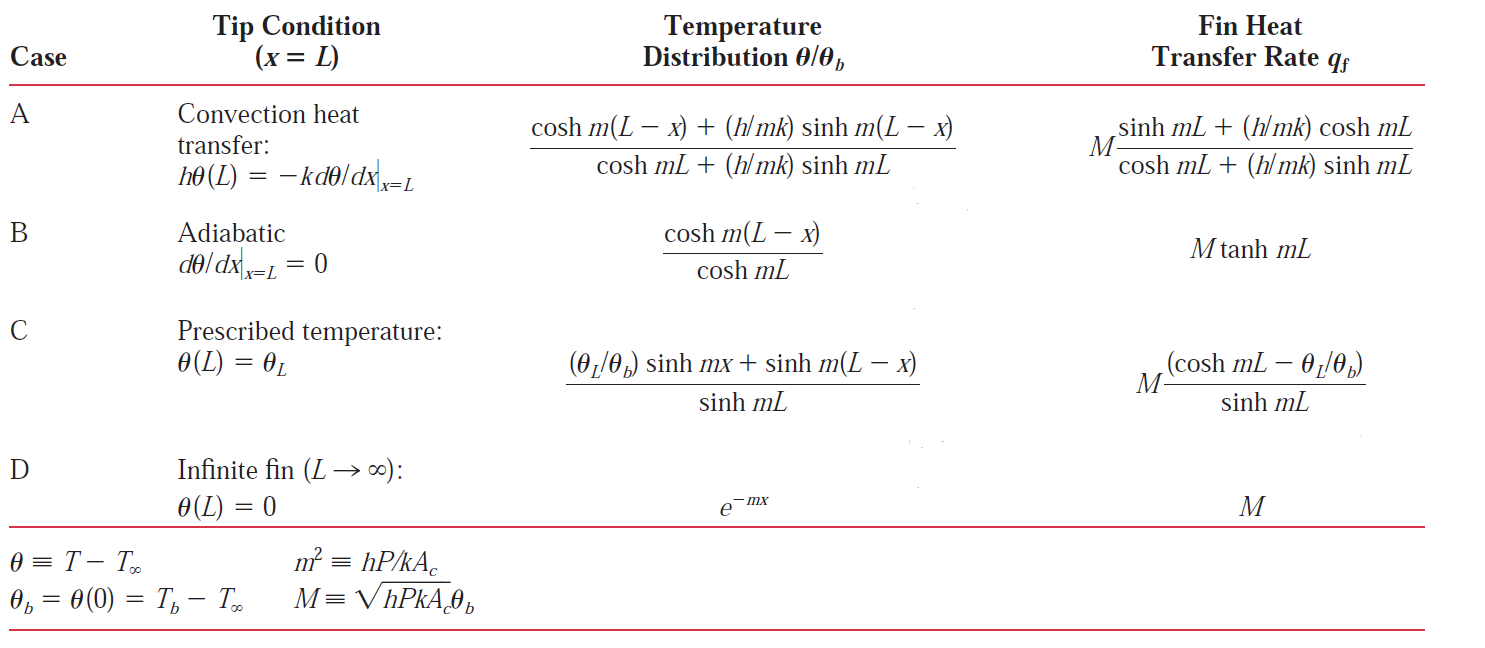
\includegraphics[width=1.0\linewidth]{images/Fin_equations.png}
        \caption{Note that P is the circumference of the cross-section element, and $A_c$ is the area of the cross-section element.}
    \end{figure}
    \item \textbf{\underline{Fin Efficiency:}} defined as the ratio of \color{red} the actual heat transfer rate from the fin \color{black} over \color{blue} ideal heat transfer rate from the fin if the entire fin were at base temperature. \color{black} 
    \begin{align*}
        \eta_{fin} &= \frac{\dot{Q}_{fin}}{\dot{Q}_{fin,max}} \\
        \dot{Q}_{fin} &= \eta_{fin} \dot{Q}_{fin,max} = \eta_{fin}h A_{fin} (T_b - T_{\infty})
    \end{align*}
    \item Corrected fin length $L_c$:
    \begin{equation*}
        L_c = L + \frac{A_c}{p}
    \end{equation*}
    \begin{figure}[H]
        \centering
        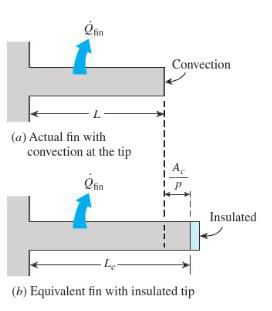
\includegraphics[width=0.6\linewidth]{images/corrected_fin_length.png}
    \end{figure}
    \item List of fin efficiency:
    \begin{figure}[H]
        \centering
        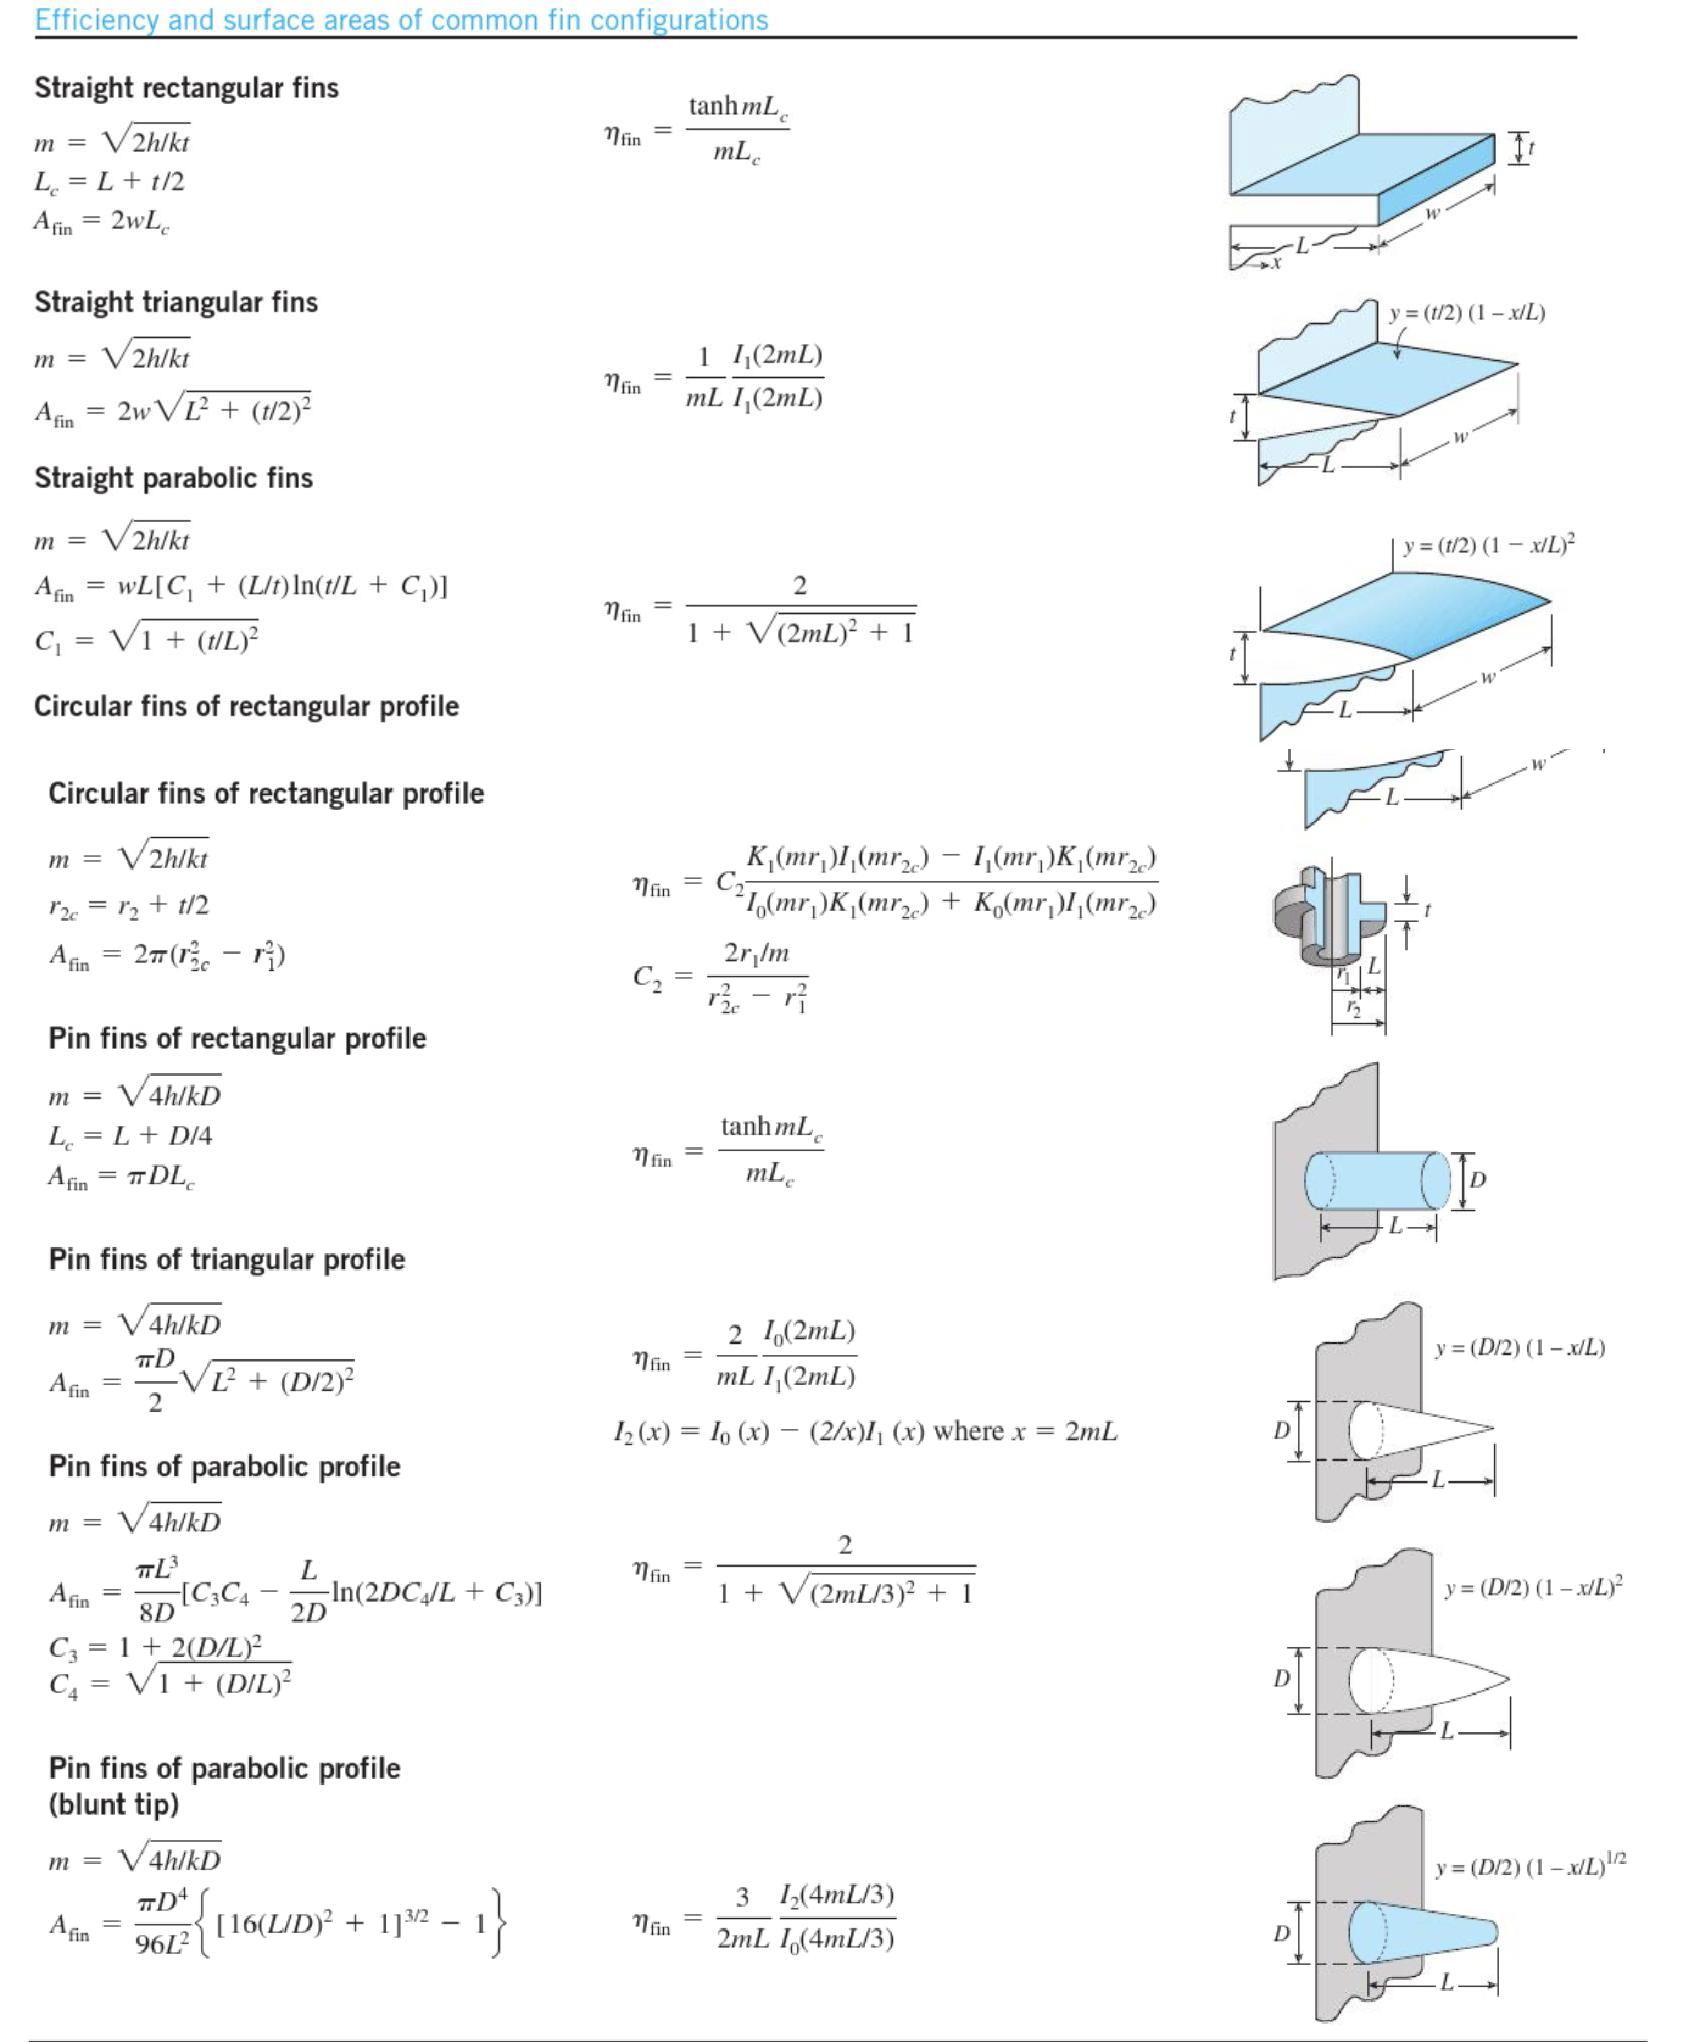
\includegraphics[width=1.0\linewidth]{images/fin_efficiency.png}
        \caption{Note $L_c$ is the corrected length.}
    \end{figure}
    \item \underline{\textbf{Fin effectiveness}}: measures the enhancement of heat transfer from fin. Defined as the ratio of \color{red} heat transfer rate from the fin of base area $A_b$ \color{black} over \color{blue} heat transfer rate from the surface of area $A_b$. \color{black}
    \begin{align*}
        \epsilon_{fin} &= \frac{\dot{Q}_{fin}}{\dot{Q}_{\text{no fin}}} = \frac{\dot{Q}_{fin}}{h A_b (T_b - T_{\infty})} \\
        &= \frac{A_{fin}}{A_b} \cdot \eta_{fin}
    \end{align*}
    \begin{figure}[H]
        \centering
        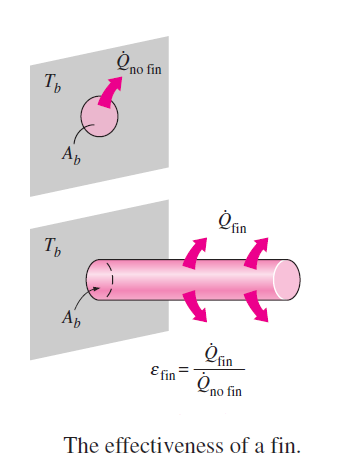
\includegraphics[width=0.5\linewidth]{images/fin_effectiveness.png}
    \end{figure}
    \begin{figure}[H]
        \centering
        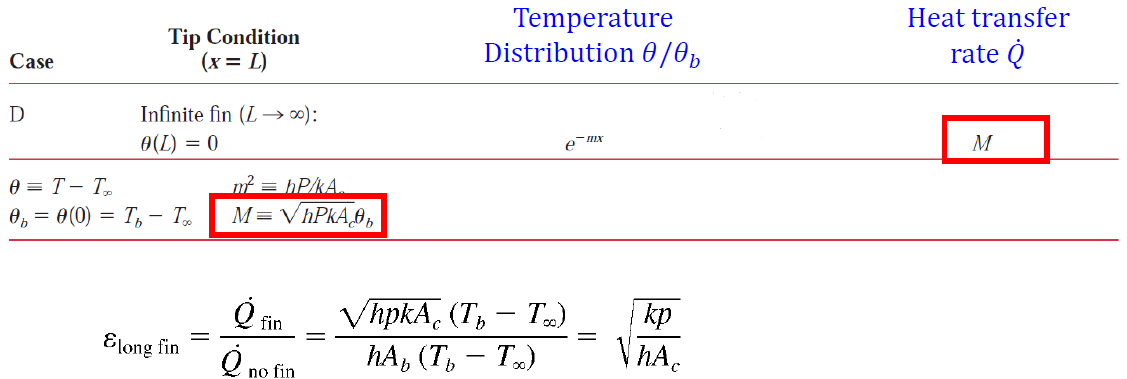
\includegraphics[width=1.0\linewidth]{images/fin_effectiveness_relation.png}
    \end{figure}
    \item $\epsilon_f \propto k$: made from metals usually;
    \item $\epsilon_f \propto \frac{1}{h}$: more effective in gases/natural convection;
    \item $\epsilon \propto \frac{P}{A_c}$: satisfied thin plate / slender fins
    \item \underline{\textbf{Fin arrays}}
    \begin{figure}[H]
        \centering
        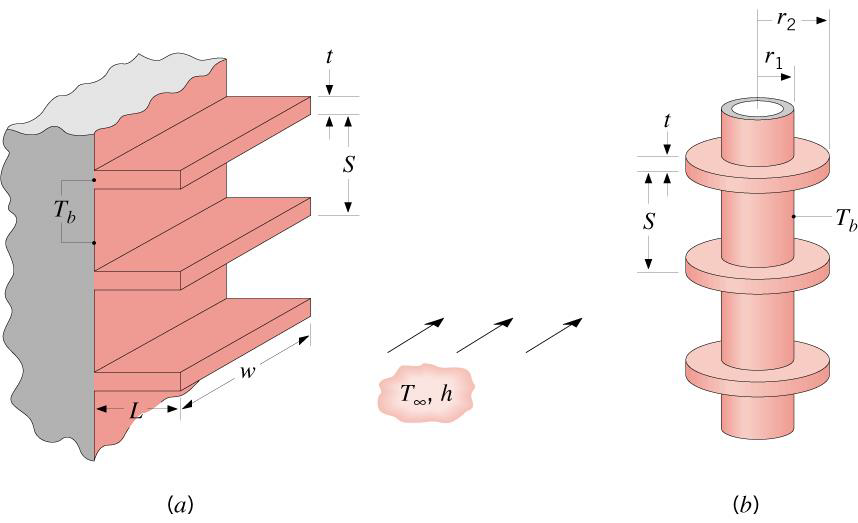
\includegraphics[width=1.0\linewidth]{images/fin_array_diagram.png}
    \end{figure}
    \begin{itemize}
        \item Total surface area:
        \begin{align*}
            A_t &= N A_f + A_b \\
            \text{where } N &= \text{number of fins,} \\
            A_b &= \text{area of exposed based (prime surface)}
        \end{align*}
        \item Total heat rate:
        \begin{align*}
            \color{blue} \dot{Q}_t &= \color{black} N \eta_f h A_f \theta_b + h A_b \theta_b \\
            &= h\left[N\eta_f A_f + (A_t - N A_f)\theta_b \right] \\
            &= h A_t \left[1 - \frac{NA_f}{A_t}(1-\eta_f)\right]
        \end{align*}
    \end{itemize}
\end{itemize}


\textbf{\underline{Fin efficiency read off from graph}}
\begin{figure}[H]
    \centering
    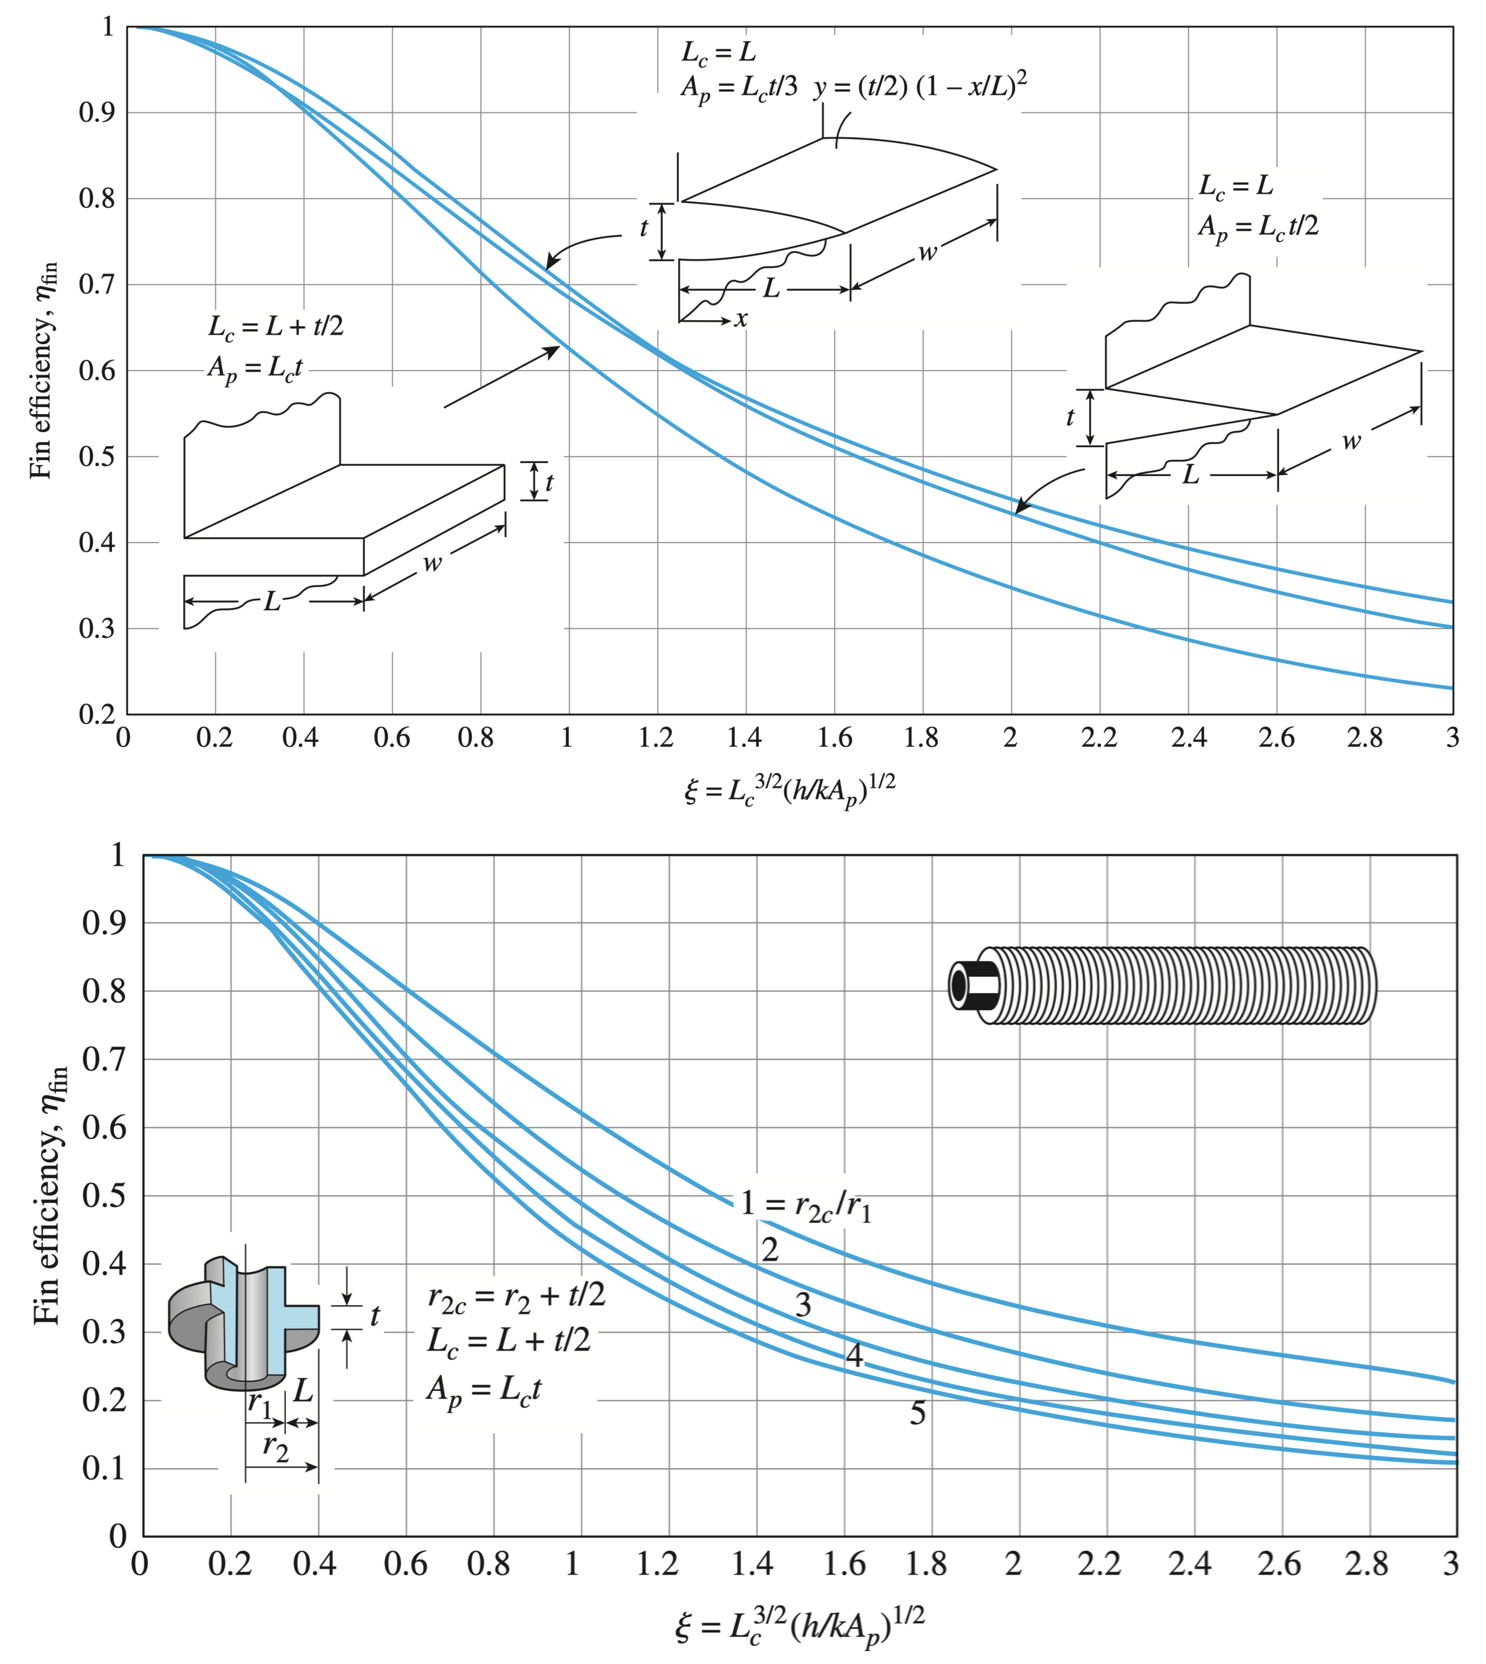
\includegraphics[width=1.0\linewidth]{images/Fin_efficiency_chart.png}
\end{figure}
Overall fin efficiency:
\begin{align*}
    R_{t,o} &= \frac{1}{\eta_o h A_t} \\
    \eta_o &= 1- \frac{N A_f}{A_t} (1-\eta_f)
\end{align*}

\textbf{\underline{Lumped Capacitance Method}}
\begin{figure}[H]
    \centering
    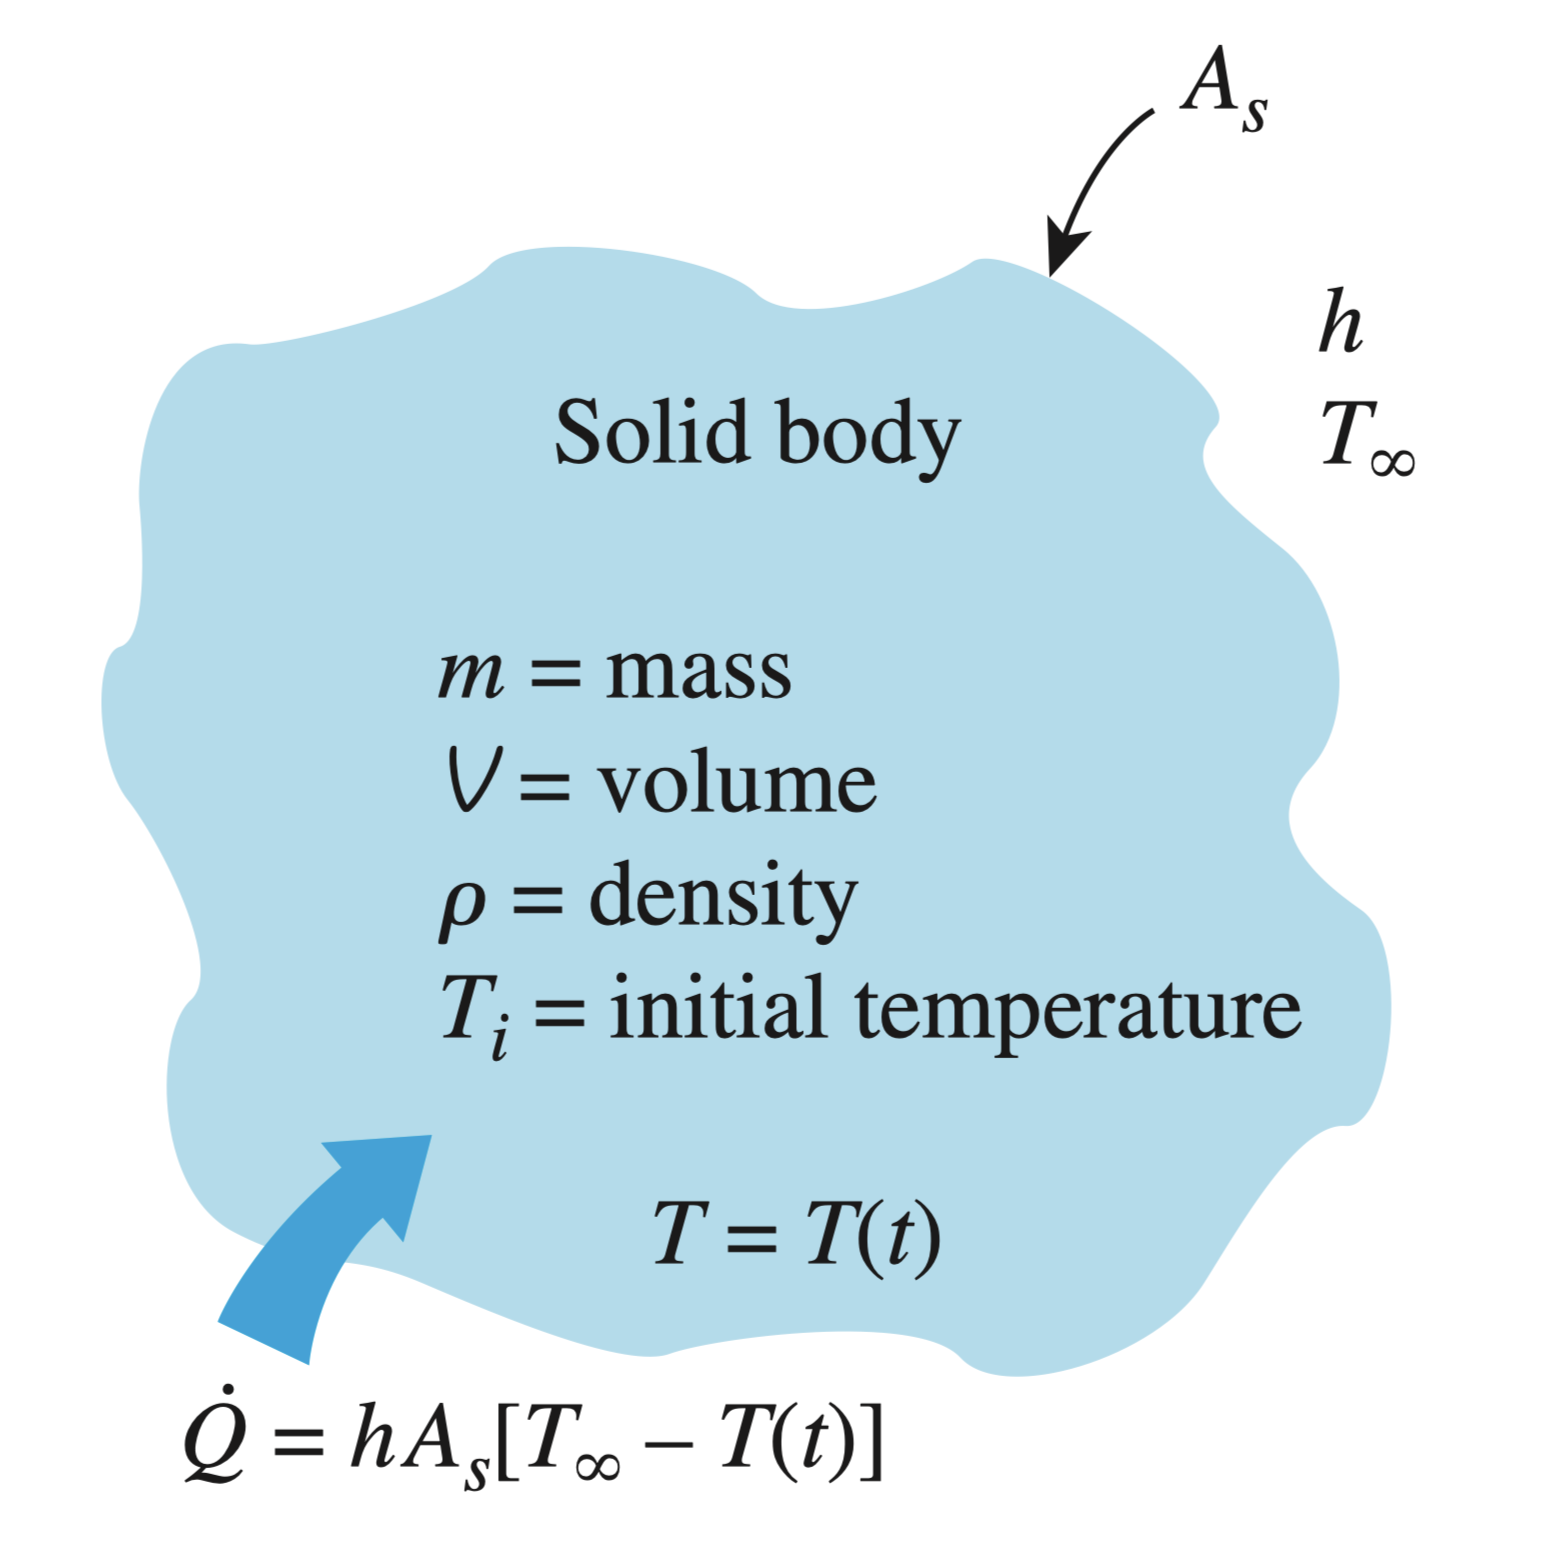
\includegraphics[width=0.55\linewidth]{images/lumped_system_analysis.png}
\end{figure}
\begin{itemize}
    \item Temperature of Body:
    \begin{align*}
        \frac{T(t) - T_{\infty}}{T_i - T_{\infty}} &= e^{-bt} \\
        \text{where } T(t) &= \text{temperature of body}\\
        b &= \frac{h A_s}{\rho V C_p} \; \text{[1/s]}
    \end{align*}
    \item Rate of heat transfer to/from environment at time t:
    \begin{equation*}
        \dot{Q}(t) = h A_s [T(t) - T_{\infty}] \;\; \; \text{[W]} 
    \end{equation*}
    \item Total amount of heat transferred between $\tau=0$ and $\tau = t$:
    \begin{equation*}
        Q = m C_p [T(t) - T_i] \;\; \; \text{[kJ]}
    \end{equation*}
    \item \textbf{\underline{Characteristic Length:}} 
    \begin{itemize}
        \item Less conservative but convenient for complex geometries: 
        \begin{equation*}
            L_c = \frac{V}{A_s} 
        \end{equation*}
        \item More conservative: calculated as the dimension corresponding to the max spatial temperature difference. Usually equivalent to \color{red} the furthest distance from surface to centroid. \color{black} 
    \end{itemize}
    \item Biot number: $\text{Bi} = \frac{h L_c}{k}$
    \begin{figure}[H]
        \centering
        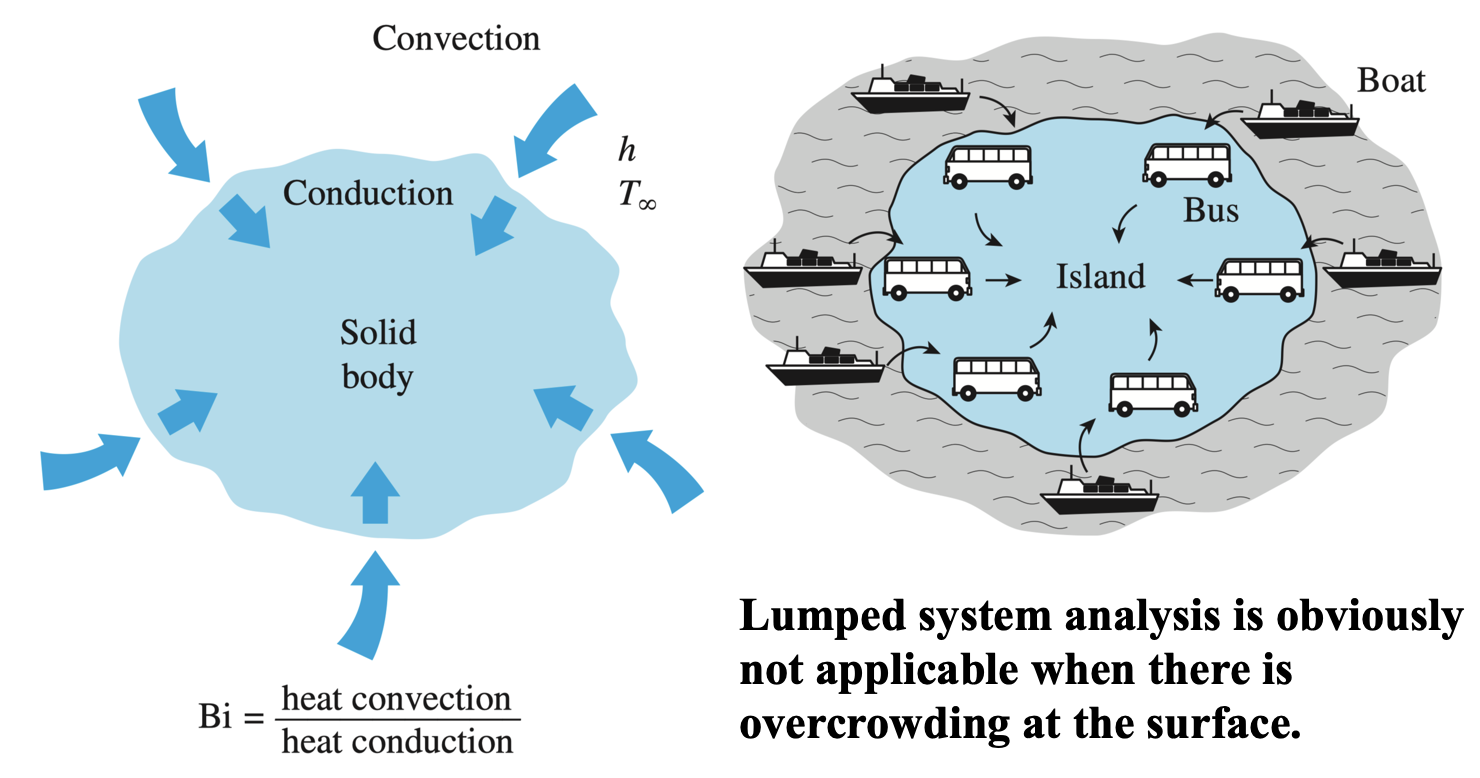
\includegraphics[width=1.0\linewidth]{images/Biot_number.png}
    \end{figure}
    \begin{itemize}
        \item Definition 1:
        \begin{align*}
            \text{Bi} &= \frac{h}{\left(\frac{k}{L_c}\right)}\cdot \frac{\Delta T}{\Delta T} \\
            &= \frac{\text{convection at the surface of body}}{\text{conduction within body}}
        \end{align*}
        \item Definition 2:
        \begin{align*}
            \text{Bi} &= \frac{\left(\frac{L_c}{k}\right)}{\left(\frac{1}{h}\right)} \\
            &= \frac{\text{conduction resistance within body}}{\text{convection resistance at the surface of body}}
        \end{align*}
    \end{itemize}
    \item \underline{Criterion for Applicability of LCM}:
    \begin{equation*}
        \text{Bi} \leq 0.1
    \end{equation*}
\end{itemize}

\underline{\textbf{\large Convections and External Flow}}
\begin{itemize}
    \item Convective heat transfer coefficient (defined at a single point):
    \begin{equation*}
        h \equiv \frac{-k_f \left(\frac{\partial T}{\partial y}\right)|_{y=0}}{T_s - T_{\infty}} \; \; \; \text{[W/$m^2\cdot K$]}
    \end{equation*}
    \item Average heat transfer coefficient (defined over the entire surface): 
    \begin{itemize}
        \item for a uniform surface temperature:
        \begin{equation*}
            \bar{h} = \frac{1}{A_s}\int_{A_s} h \, d A_s
        \end{equation*}
        \item for a flat plate in parallel flow:
        \begin{equation*}
            \bar{h} = \frac{1}{L} \int_{0}^{L} h \, dx
        \end{equation*}
    \end{itemize}
    
    
    \item \underline{\textbf{\large Nußelt number (non-dimensional)}}
    \begin{figure}[H]
        \centering
        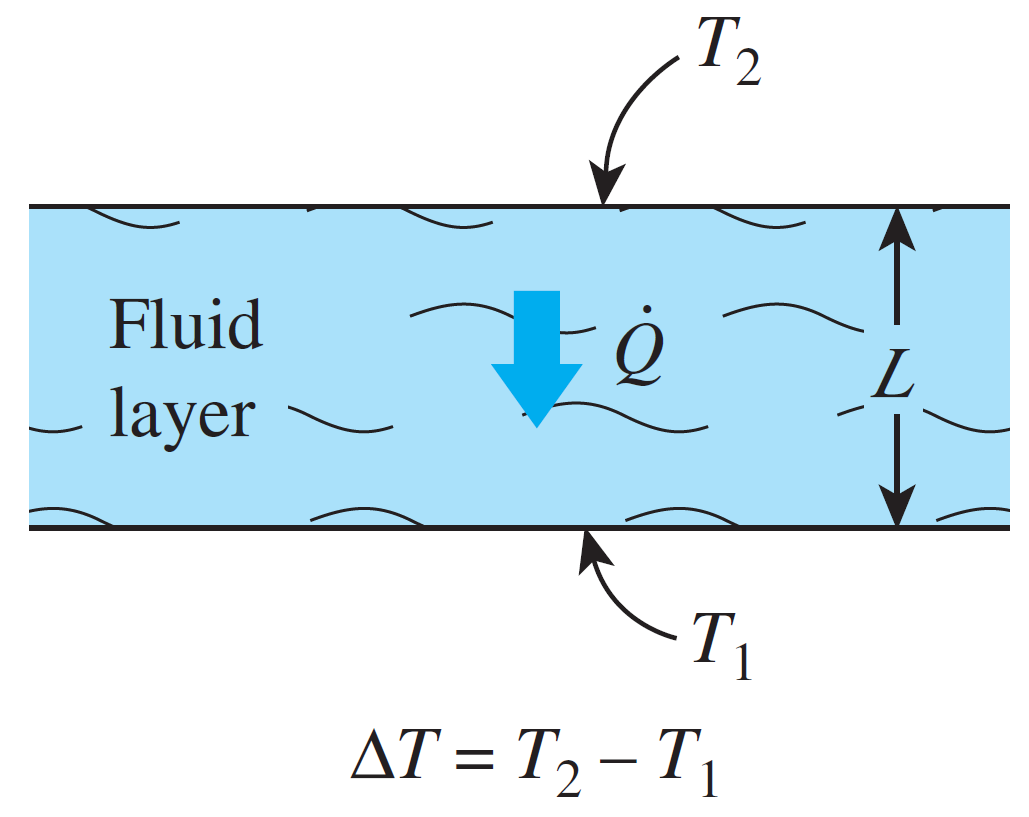
\includegraphics[width=0.55\linewidth]{images/Nusselt_number.png}
    \end{figure}
    \begin{equation*}
        \frac{q^{''}_{conv}}{q^{''}_{cond}} = \frac{h \Delta T}{k \left(\frac{\Delta T}{L_c}\right)} = \frac{hL_c}{k} = \text{Nu}
    \end{equation*}
    \item \textbf{Nu}: enhancement of heat transfer due to convection relative to conduction across the same fluid layer.
    \begin{itemize}
        \item $\text{Nu}>1$: (usually in laminar flows) the more effective convective heat transfer.
        \item $\text{Nu}\gg 1$: (usually in turbulent flows) 
        \item $\text{Nu}=1$: heat transfer is pure conduction
        \item $\text{Nu}<1$: Not possible. Convection always increases heat transfer.
    \end{itemize}
\end{itemize}